\documentclass[letterpaper,10pt,twocolumn]{article}

\usepackage[spanish]{babel}
\usepackage{amsmath}
\usepackage{graphics}
\usepackage{abstract}
\usepackage{graphicx}
%opening
\title{Power Spectral Density Calculations}
\author{Roberto Casta\~neda Sheissa}
\begin{document}

\maketitle

\begin{abstract}
Se muestra la manera en que se obtienen las f\'ormulas para realizar el c\'alculo del valor de \textbf{potencia de densidad espectral}. La f\'ormula general ya es conocida sin embargo es posible caer en errores cuando se quiere aplicar; sobre todo si se manejan las unidades $\frac{X}{\sqrt{Hz}}$ (X puede ser {\bf voltaje} o {\bf corriente}). La correcta aplicaci\'on de la f\'ormula garantizar\'a que los valores obtenidos de las ecuaciones puedan ser corroborados por medio de alg\'un paquete de simulaci\'on de circuitos (\it{ PSPICE, HSPICE, topSPICE, etc}). 
\end{abstract}

\section{Introducci\'on}
Con respecto al ruido una red de amplificaci\'on se comporta de forma lineal, tal que puede describirse la contribuci\'on de cada fuente ruidosa con respecto a la fuente equivalente de ruido en la entrada del amplificador como una convoluci\'on (en el dominio del tiempo) con una respuesta impulso $h_k(\tau)$. Si se reservan los \'indices {\it impares} para las fuentes ruidosas de corriente y los {\it pares} para las fuentes ruidosas de voltaje, formalmente se puede expresar la fuente equivalente de ruido en la entrada (ya sea voltaje o corriente) de la siguiente forma:
\begin{equation} \label{eq:eq1}
e_{n,in}(t)=\sum_{i=1}^nh_{2i}*v_{n,2i}(t)+\sum_{k=0}^mh_{2k+1}*i_{n,2k+1}(t)
\end{equation}
donde "*" denota {\it convoluci\'on}.
cuando un proceso ruidoso $e_{n,y}(t)$ es igual a la convoluci\'on de una respuesta-impulso invariante en tiempo lineal $h(\tau)$ y un proceso ruidoso $e_{n,x}(t)$, esto es 
\begin{equation}
e_{n,y}(t)=h*e_{n,x}(t) 
\end{equation}
entonces su potencia de densidad espectral $S_{n,y}(f)$ se relaciona con la potencia de densidad espectral $S_{n,x}(f)$ de $e_{n,x}(t)$ por medio de la ecuaci\'on:
\begin{equation}
S_{n,y}(f)=\lvert H(j2\pi f)\rvert^{2}S_{n,x}(f)
\end{equation}
donde la funci\'on de transferencia $H(j2\pi f)$ es la transformada de Fourier a $h(\tau)$. Aplicando este teorema a la ecuaci\'on (\ref{eq:eq1}) se puede observar que la potencia de densidad espectral del ruido equivalente a la entrada puede ser expresada por:
\begin{equation}
\begin{split}
S_{n,in}=\sum_{i=1}^n{\lvert}H_{2i}(j2{\pi}f){\rvert}^2S_{v_{n,2i}}(f)+\\
\sum_{k=0}^m{\lvert}H_{2k+1}(j2{\pi}f){\rvert^2}S_{i_{n,2k+1}}(f)
\end{split}
\end{equation} 
La potencia de densidad espectral de un proceso el\'ectrico ruidoso es dado com\'unmente en t\'erminos del valor medio cuadr\'atico del ruido asociado a una banda de frecuencia $[f,f+{\Delta}f]$. Este valor es nada mas que la potencia contenida en una banda de frecuencia ${\Delta}f$ alrededor de una frecuencia $f$. En consecuencia si $\overline{v_n^2}(f,{\Delta}f)$ representa el valor medio cuadr\'atico de un voltaje ruidoso $v_n(t)$ en una banda de frecuencia ${\Delta}f$ alrededor de $f$, y $S_{v_n}(f)$ representa la densidad de potencia espectral asociada, entonces la relaci\'on entre los dos est\'a dada por:
\begin{equation}
S_{v_n}(f)=\lim_{{\Delta}f \to 0}\frac{\overline{v_n^2}(f,{\Delta}f)}{{\Delta}f}
\end{equation}
en el caso de obtener la corriente se utiliza la misma f\'ormula, \'unicamente es necesario sustituir {\it v} por {\it i}.

\section{Aplicaci\'on}
La teor\'ia anteriormente detallada se aplicar\'a a un amplificador de voltaje utilizando un dispositivo BJT como s\'inteis del nullor en primera etapa. La figura \ref{fig:noisebjt} muestra el modelo de ruido para el transistor bipolar.

\begin{figure}
   \centering
   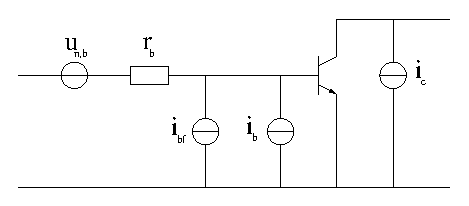
\includegraphics[scale=1]{/home/roberto/Pre_docs/figuras/bjt_noisemodel.eps}
   \caption{BJT noise model}
   \label{fig:noisebjt}
\end{figure}

El amplificador de voltaje utiliza retroalimentaci\'on negativa directa como la que se muestra en la figura \ref{fig:voltamp}. En este caso la red de retroalimentaci\'on consistir\'a de dos resistencias figura \ref{fig:null_voltamp}.

\begin{figure}
   \centering
   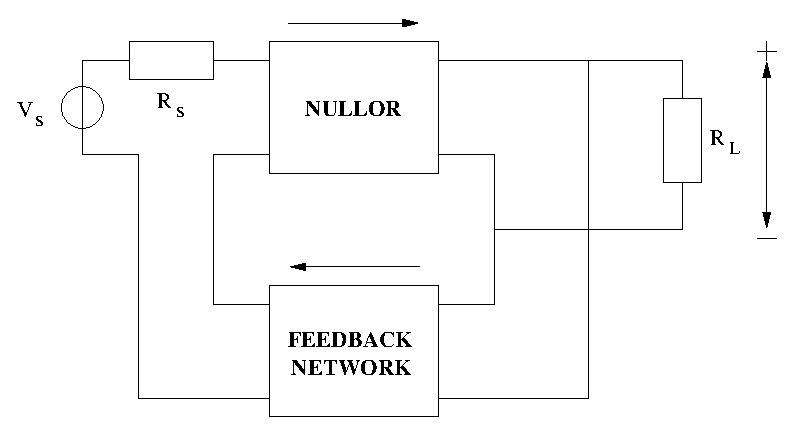
\includegraphics[scale=.5]{/home/roberto/Pre_docs/figuras/direct_voltamp.eps}
   \caption{Amplificador de voltaje con retroalimentaci\'on negativa}
   \label{fig:voltamp}
\end{figure}

\begin{figure}
   \centering
   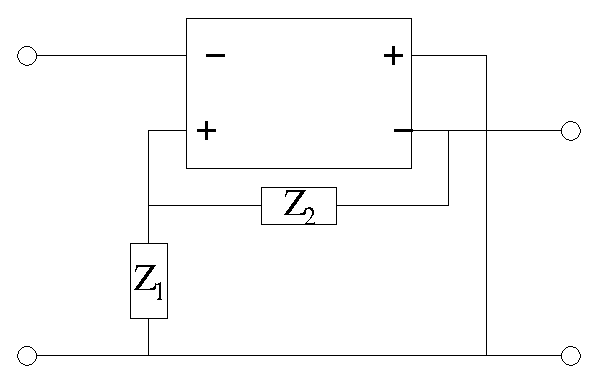
\includegraphics[scale=.5]{/home/roberto/Pre_docs/figuras/voltaje_amp.eps}
   \caption{Amplificador de voltaje con nullor.}
   \label{fig:null_voltamp}
\end{figure}

La configuraci\'on m\'as com\'un para obtener el nivel mas bajo de ruido en la entrada del amplificador es {\bf emisor com\'un}. Bas\'andose en esta configuraci\'on se llega a la topolog\'ia que se muestra en la figura \ref{fig:bjt_voltamp}.

\begin{figure}
   \centering
   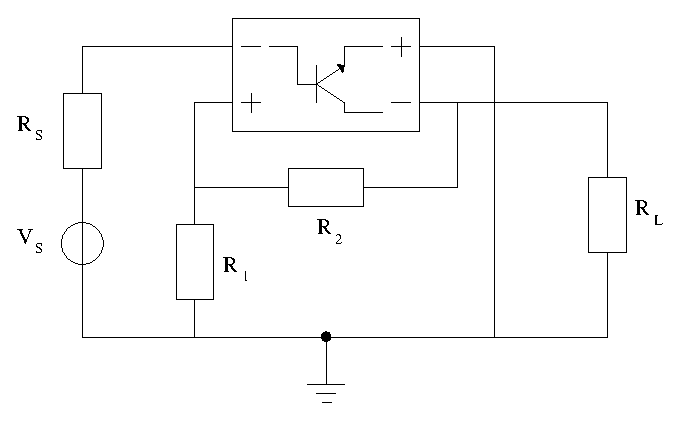
\includegraphics[scale=.5]{/home/roberto/Pre_docs/figuras/bjt_voltamp.eps}
   \caption{Amplificador de voltaje con BJT en la entrada.}
   \label{fig:bjt_voltamp}
\end{figure}

Una vez definida la topolog\'ia del circuito se introducen las fuentes de ruido que contiene el circuito. Al agreagar las fuentes de ruido al circuito se pueden hacer dos cosas. La primera es el agregar las fuentes de ruido sin tomar en cuenta las fuentes de ruido introducidas por el dispositivo BJT, por separado se agregan las fuentes de ruido de acuerdo al modelo de la figura \ref{fig:noisebjt}, una vez hecho esto estas se van reduciendo de tal forma que \'unicamente se obtengan dos fuentes ruidosas, de voltaje y corriente. La segunda opci\'on es el agregar {\bf todas} las fuentes de ruido en el circuito; esta forma es un poco m\'as complicada y puede provocar errores al reducir las fuentes. En este trabajo utilizaremos la primer forma.

\section{Desarrollo}
La ecuaci\'on de ruido para el amplificador de voltaje con retroalimentaci\'on negativa es:
\begin{equation}\\
\begin{split}
u_{n,v_{total}}=u_{ns}+u_{nn}+\biggl(R_s+\frac{R_1R_2}{R_1+R_2}\biggr)i_{nn}+\\
\biggl(\frac{R_2}{R_1+R_2}\biggr)u_{nR_1}+\biggl(\frac{R_1}{R_1+R_2}\biggr)u_{nR_2}
\end{split}
\end{equation}
donde $u_{ns}$ es el voltaje de ruido provocado por la resistencia de la fuente de excitaci\'on, $u_{nn}$ es el voltaje de ruido asociado al nullor; sin embargo dadas las caracter\'isticas ideales del nullor, no existe contribuci\'on de ruido. Al realizar la s\'intesis del nullor los elementos activos utilizados para este fin no son ideales por lo tanto existir\'a una contribuci\'on de ruido tanto de voltaje como de corriente, esta contribuci\'on se toma en cuenta por el t\'ermino $i_{nn}$. El voltaje de ruido provocado por las resistencias $R_1$ y $R_2$ est\'an dadas por $u_{nR_1}$ y $u_{nR_2}$ respectivamente.

Los valores de ruido de las resistencias est\'an dados por la ecuaci\'on
\begin{equation}
\overline{v_n^2}(f,{\Delta}f)=4kTR{\Delta}f
\end{equation}
donde $k$ es la constante de Boltzmann, $T$ es la temperatura en grados Kelvin y ${\Delta}f$ es el ancho de banda en que trabajar\'a el circuito. En cuanto al dispositivo BJT las contribuciones est\'an dadas por la siguientes relaciones:
\begin{align}
\overline{i_c^2}(f,{\Delta}f)&=2qI_c{\Delta}f, f\geq0\\
\overline{i_b^2}(f,{\Delta}f)&=2qI_b{\Delta}f, f\geq0\\
\overline{u_{nb}^2}(f,{\Delta}f)&=4kTr_b{\Delta}f, f\geq0
\end{align}
siendo los t\'erminos $I_c$ e $I_b$ los valores en DC de las corrientes de colector y base respectivamente. El t\'ermino $u_{nb}$ se refiere al ruido t\'ermico generado por la resistencia de base, dado que este valor es el mayor (generalmete) en el transistor su contribuci\'on no puede ser despreciada. Existe otra contribuci\'on al ruido del transistor, es el ruido {\it flicker} debido a una variedad de imperfecciones del semiconductor. Al contrario que las tres contribuciones mencionadas anteriormente, dado que la frecuencia de {\it flicker} para el transistor actual es de unos pocos Hertz la contribuci\'on total al ruido puede ser despreciada.

Por medio de una transformaci\'on de dos puertos es posible colocar la fuente de ruido de corriente en la base del transistor, por la configuraci\'on de emisor com\'un. Este movimiento debe de respetar las reglas para dos puertos. Ahora el modelo del transistor queda de la siguiente forma (figura \ref{fig:bjt_noise1}).
\begin{figure}
   \centering
   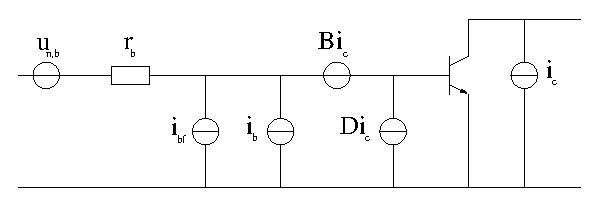
\includegraphics[scale=.7]{/home/roberto/Pre_docs/figuras/bjt_noisemodel1.eps}
   \caption{Modelo de ruido para BJT emisor com\'un.}
   \label{fig:bjt_noise1}
\end{figure}
Los par\'ametros {\bf B} y {\bf D} de la matriz de la cadena para esta configuraci\'on son:
$$ B=\frac{1}{g_m}\quad D=\frac{1}{\beta}$$ 

N\'otese que aunque se coment\'o que la contribuci\'on de ruido {\it flicker} por lo regular es despreciable se incluy\'o en la figura en el caso que dicha contribuci\'on deba (o quiera) tomarse en cuenta. Dada la topolog\'ia en que se encuentran las fuentes de corriente con respecto a la resistencia de base, se procede a aplicar transformaciones Th\'evenin-Norton sobre dichas fuentes para tomar en cuenta las contribuciones de ruido por voltaje. El circuito queda finalmente como se muestra en la figura \ref{fig:bjt_noise2}.
\begin{figure}
   \centering
   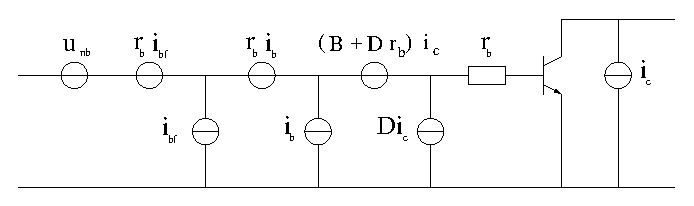
\includegraphics[scale=.7]{/home/roberto/Pre_docs/figuras/bjt_noisemodel2.eps}
   \caption{Modelo BJT con todas las fuentes de ruido.}
   \label{fig:bjt_noise2}
\end{figure}

\end{document}